\chapter{Requirement Analysis}

\section{Introduction}
This chapter presents a comprehensive analysis of the requirements for the Quantum Virtual Machine (QVM) system. The requirements were gathered through a combination of literature review, analysis of existing quantum computing frameworks, and iterative prototyping. The chapter defines the functional and non-functional requirements that guided the system's design and implementation, ensuring that the QVM achieves its goal of providing a hardware-agnostic quantum execution runtime.

\section{Requirement Elicitation Techniques}
The requirements for the QVM were elicited using multiple complementary techniques to ensure comprehensive coverage of system needs:

\textbf{Literature Review:} Extensive analysis of academic papers and technical documentation from major quantum computing frameworks (Qiskit, Cirq, ProjectQ) to identify industry standards and best practices for quantum compilation and simulation.

\textbf{Comparative Analysis:} Systematic comparison of existing quantum SDKs to identify gaps in portability, educational accessibility, and hardware abstraction that the QVM aims to address.

\textbf{Prototyping and Iteration:} Incremental development approach where initial prototypes revealed technical constraints and user needs, leading to refined requirements for classical memory integration, control flow support, and transpilation strategies.

\textbf{Domain Expert Consultation:} Regular discussions with the FYP supervisor and review of quantum computing research to validate technical requirements and ensure alignment with quantum computing principles.

\section{User Classes and Characteristics}

\begin{table}[H]
\centering
\caption{User Classes and Characteristics}
\begin{tabular}{|p{3cm}|p{5cm}|p{5cm}|}
\hline
\textbf{User Class} & \textbf{Description} & \textbf{Characteristics} \\
\hline
Quantum Algorithm Developers & Users who write and test quantum algorithms & Technical background in quantum computing; need hardware abstraction; require visualization and debugging tools \\
\hline
Students and Educators & Academic users learning quantum computing concepts & Beginner to intermediate technical skills; need clear documentation; require educational examples and visual feedback \\
\hline
Researchers & Users conducting quantum computing research & Advanced technical skills; need flexibility and extensibility; require accurate simulation and performance metrics \\
\hline
System Integrators & Users integrating QVM with other tools & Software engineering background; need API access; require export capabilities (OpenQASM) \\
\hline
\end{tabular}
\end{table}

\section{System Overview}
The Quantum Virtual Machine is a comprehensive quantum circuit execution platform that implements a complete compilation and simulation pipeline. The system accepts quantum programs in multiple formats (OpenQASM 2.0, OpenQASM 3.0, JSON), transforms them through a hardware-agnostic intermediate representation, applies topology-aware transpilation, and executes them using either exact statevector simulation or efficient tensor network methods. The system provides three user interfaces (CLI, Web API, Web GUI) to accommodate different usage scenarios, from automated scripting to interactive exploration. The architecture emphasizes modularity, allowing each component (parser, transpiler, simulator) to be independently tested and upgraded.

\section{Use Case Model}
This section defines the primary interactions between the actors and the Quantum Virtual Machine system, capturing the functional requirements from a user-centric perspective.

\subsection{Combined Use Case Diagram}
The use case diagram in Figure \ref{fig:use_case_diagram} provides a high-level visual overview of the system's functionality and all actors involved.

\begin{figure}[H]
\centering
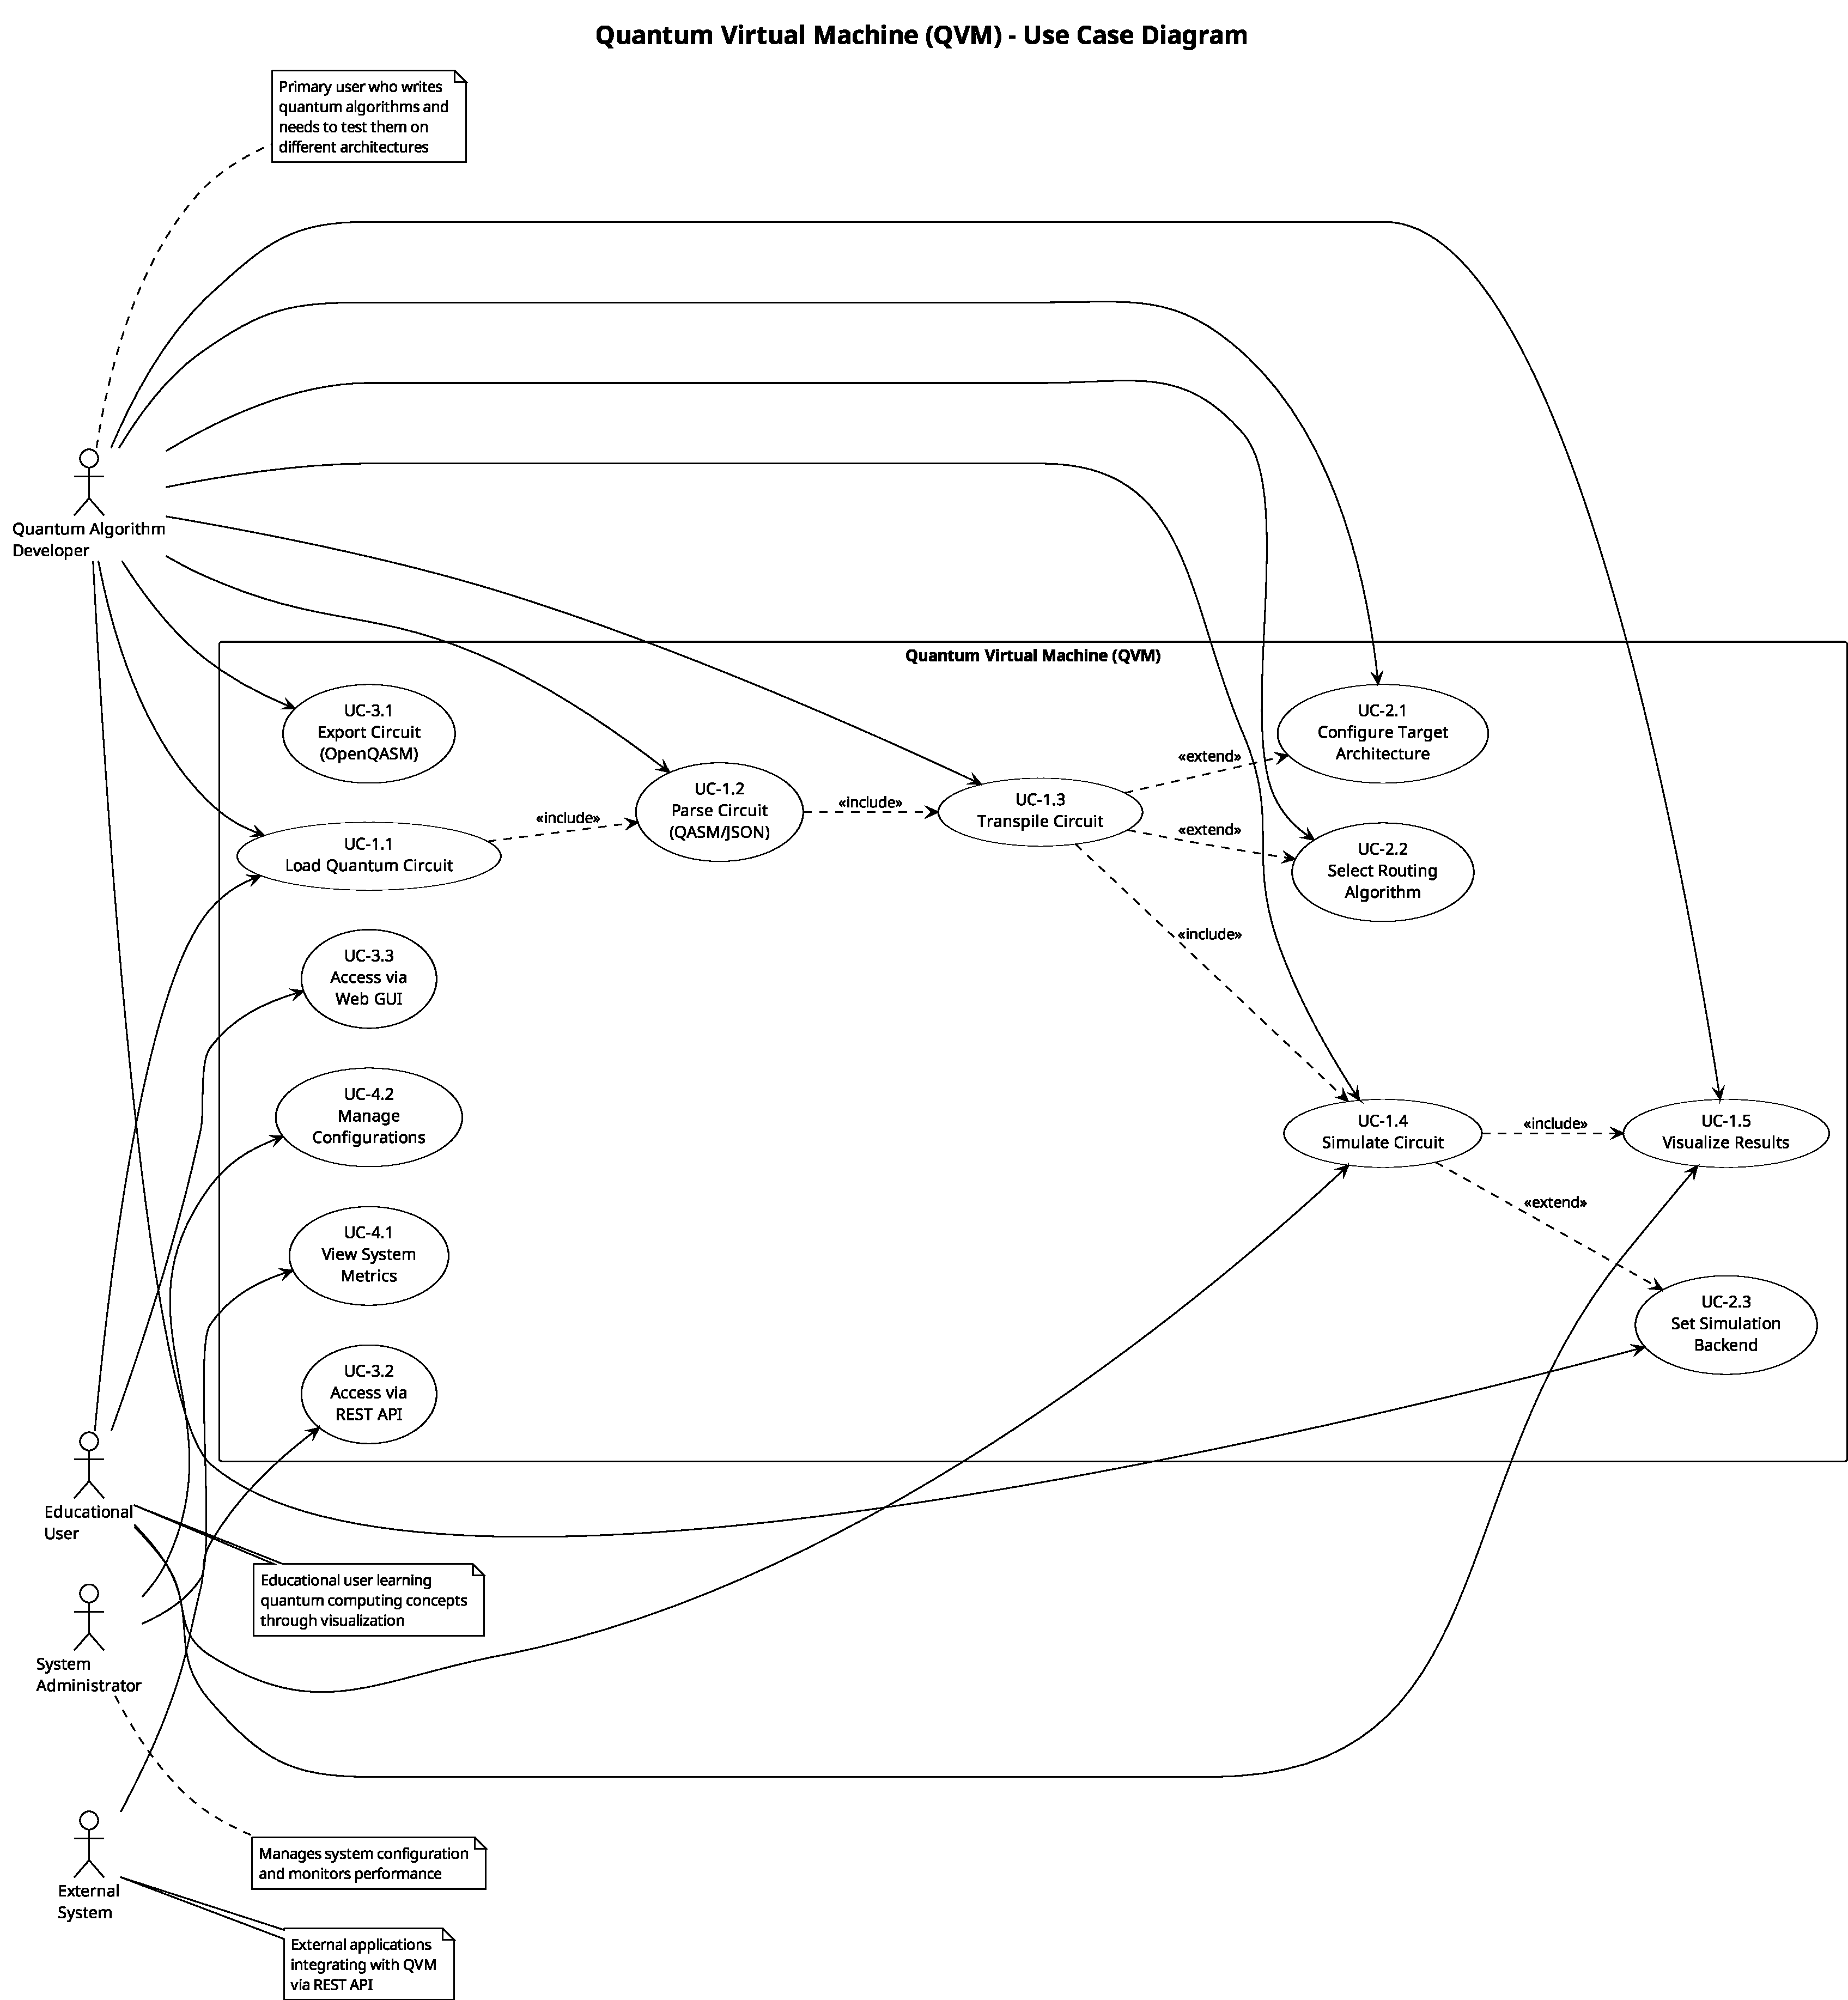
\includegraphics[width=0.9\textwidth,height=0.8\textheight,keepaspectratio]{../uml/QVM_Use_Case_Diagram.pdf}
\caption{Combined Use Case Diagram for Quantum Virtual Machine}
\label{fig:use_case_diagram}
\end{figure}

\subsection{Actor-Specific Use Case Diagrams}
The following diagrams present individual use case views for each distinct user class, showing the specific interactions and system capabilities relevant to each actor.

\subsubsection{Quantum Algorithm Developer}
Figure \ref{fig:uc_developer} illustrates the use cases available to the Quantum Algorithm Developer. This actor is the primary user of the system, interacting with the QVM to parse, transpile, simulate, and visualize quantum circuits via the command-line interface.

\begin{figure}[H]
\centering
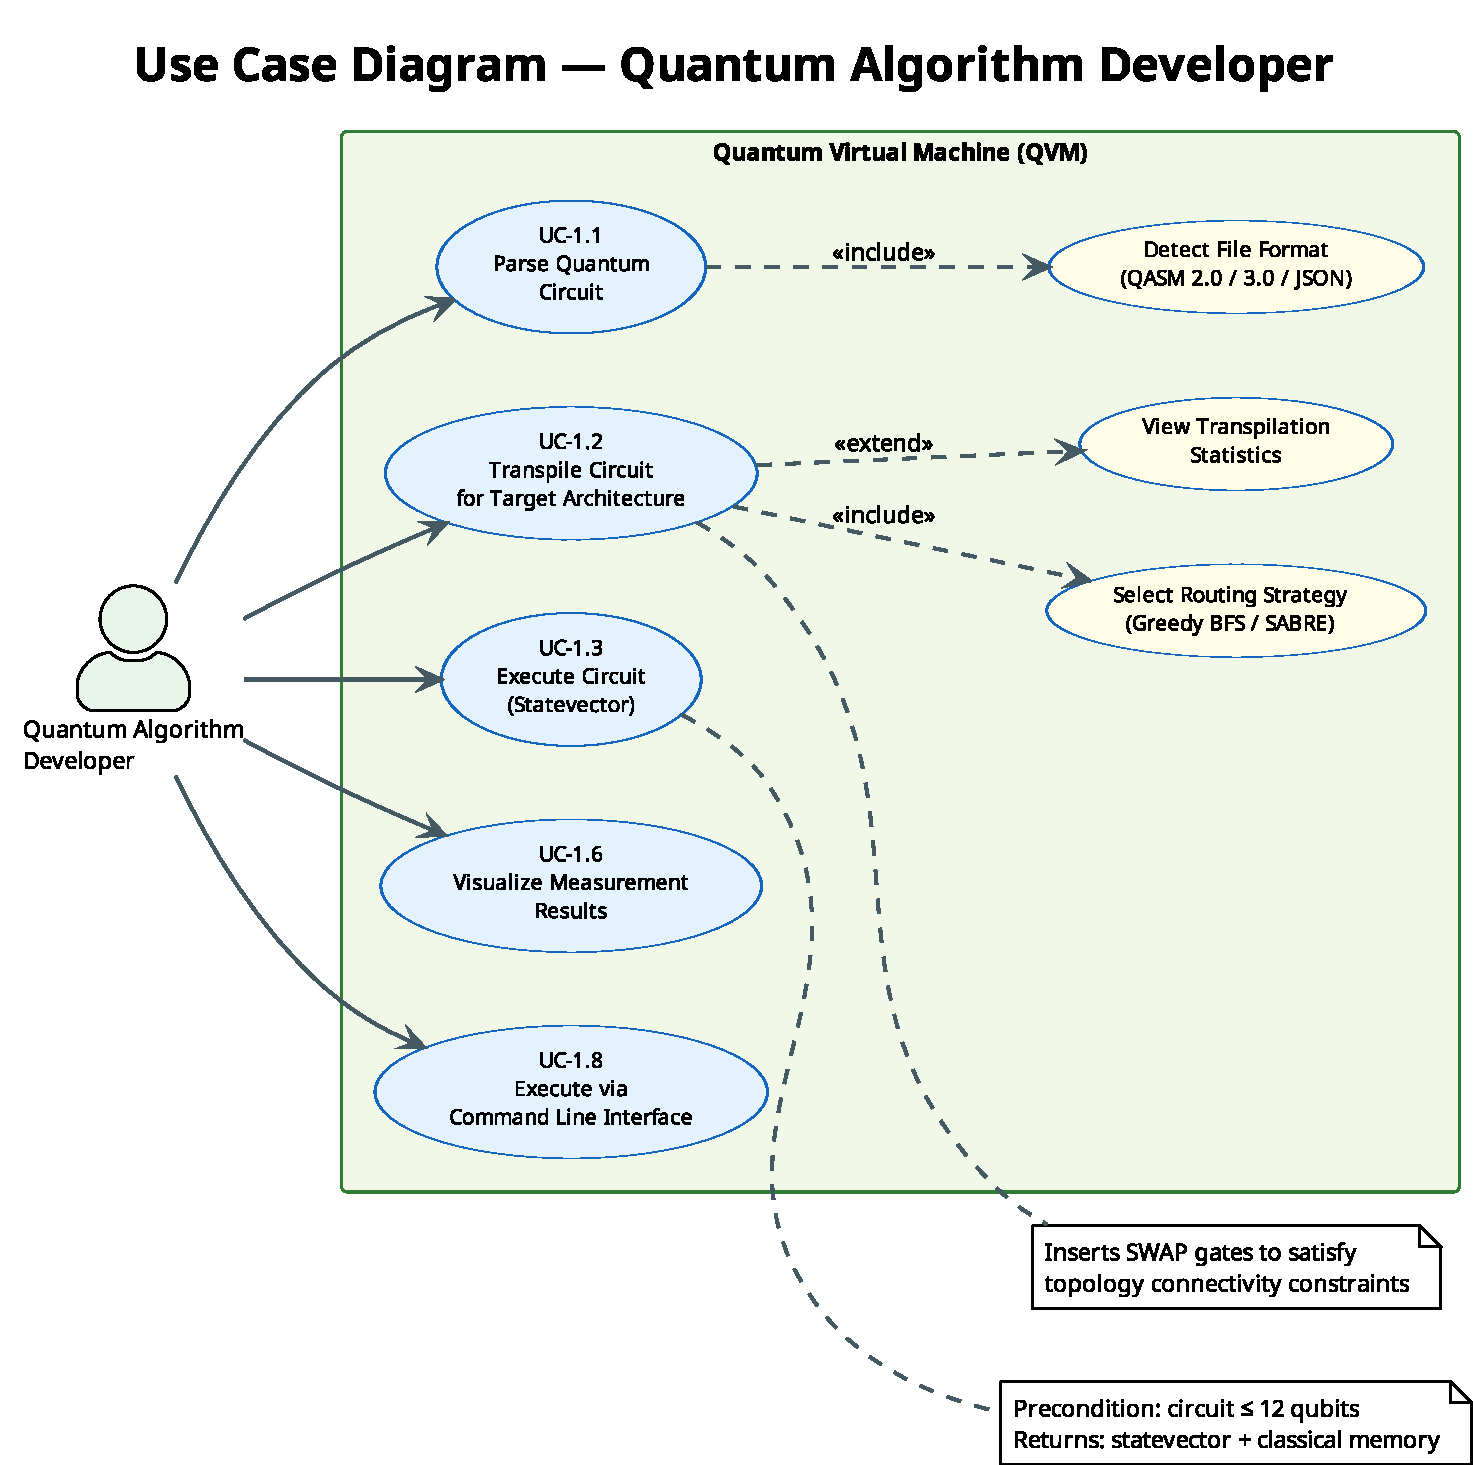
\includegraphics[width=0.9\textwidth,height=0.75\textheight,keepaspectratio]{../standalone_docs/figures/UC_Developer.pdf}
\caption{Use Case Diagram --- Quantum Algorithm Developer}
\label{fig:uc_developer}
\end{figure}

\subsubsection{Student / Educator}
Figure \ref{fig:uc_student} shows the use cases for the Student / Educator actor. This user class interacts primarily with the web-based GUI and visualization features to learn quantum computing concepts through experimentation.

\begin{figure}[H]
\centering
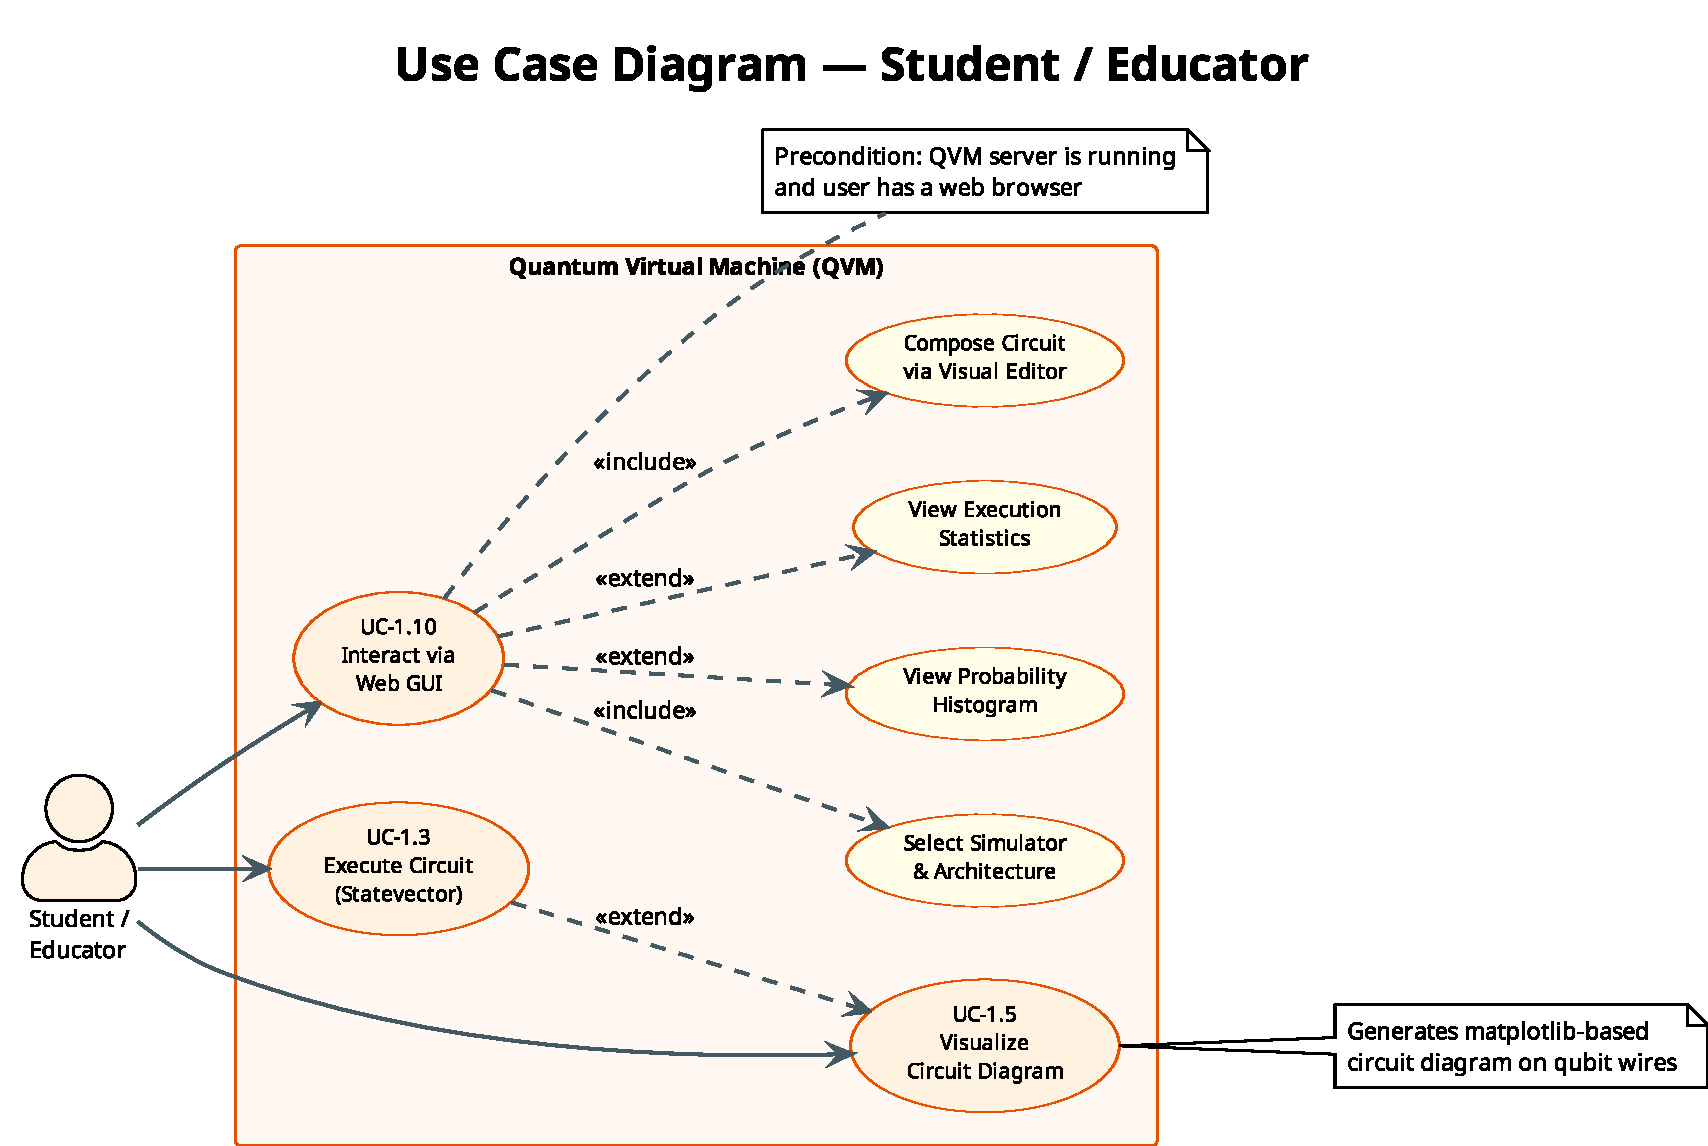
\includegraphics[width=0.9\textwidth,height=0.6\textheight,keepaspectratio]{../standalone_docs/figures/UC_Student.pdf}
\caption{Use Case Diagram --- Student / Educator}
\label{fig:uc_student}
\end{figure}

\subsubsection{Researcher}
Figure \ref{fig:uc_researcher} presents the use cases for the Researcher actor. This user class requires advanced simulation capabilities, including the MPS simulator and detailed transpilation benchmarking.

\begin{figure}[H]
\centering
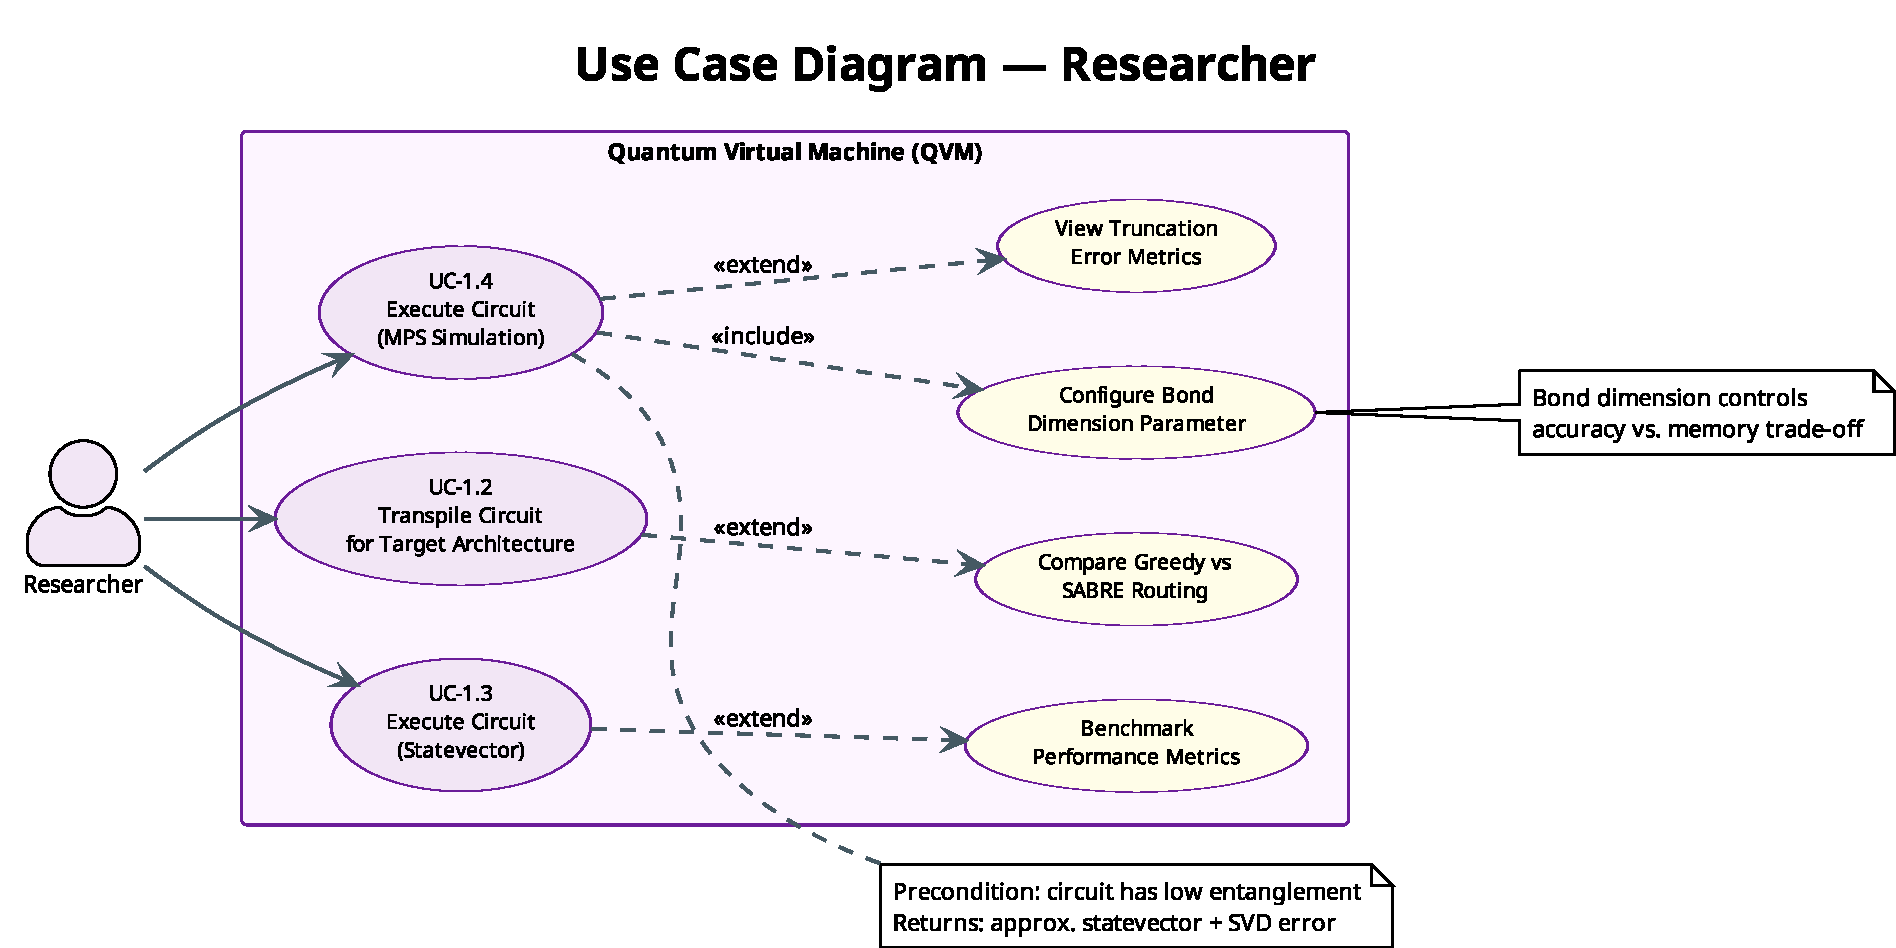
\includegraphics[width=0.9\textwidth,height=0.5\textheight,keepaspectratio]{../standalone_docs/figures/UC_Researcher.pdf}
\caption{Use Case Diagram --- Researcher}
\label{fig:uc_researcher}
\end{figure}

\subsubsection{System Integrator}
Figure \ref{fig:uc_integrator} depicts the use cases for the System Integrator actor. This actor accesses the QVM programmatically via the REST API or exports circuits in OpenQASM format for use with external quantum platforms.

\begin{figure}[H]
\centering
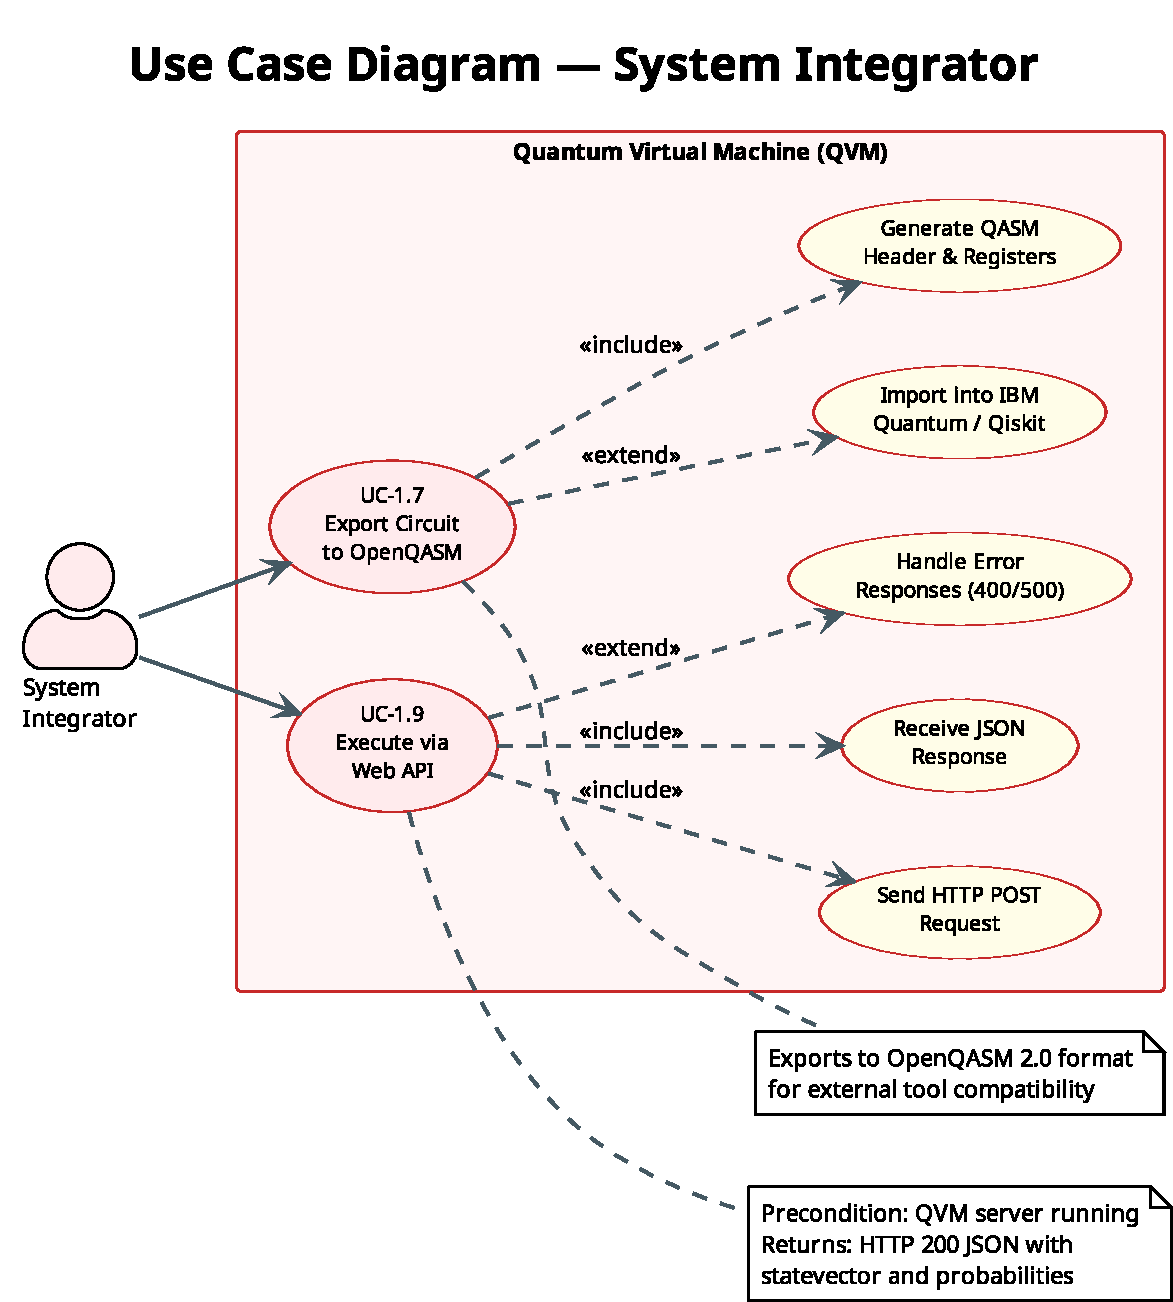
\includegraphics[width=0.9\textwidth,height=0.65\textheight,keepaspectratio]{../standalone_docs/figures/UC_Integrator.pdf}
\caption{Use Case Diagram --- System Integrator}
\label{fig:uc_integrator}
\end{figure}

\subsection{Use Case Descriptions}
The following descriptions provide detailed step-by-step flows for each use case identified in the diagram, including preconditions, main flows, and alternative paths.

\textbf{UC-1.1: Parse Quantum Circuit}
\begin{itemize}
\item \textbf{Actor:} Quantum Algorithm Developer
\item \textbf{Description:} User provides a quantum circuit in OpenQASM or JSON format, and the system parses it into an internal intermediate representation.
\item \textbf{Preconditions:} Valid circuit file exists
\item \textbf{Postconditions:} QuantumCircuit IR object is created
\item \textbf{Main Flow:}
\begin{enumerate}
\item User provides circuit file path
\item System detects file format (QASM 2.0, QASM 3.0, or JSON)
\item System invokes appropriate parser
\item Parser validates syntax and semantics
\item System creates QuantumCircuit IR object
\item System returns success confirmation
\end{enumerate}
\item \textbf{Alternative Flows:}
\begin{itemize}
\item 4a. Syntax error detected: System reports error with line number and description
\item 4b. Semantic error detected: System reports invalid gate or qubit reference
\end{itemize}
\end{itemize}

\textbf{UC-1.2: Transpile Circuit for Target Architecture}
\begin{itemize}
\item \textbf{Actor:} Quantum Algorithm Developer
\item \textbf{Description:} User requests transpilation of a logical circuit to match a specific hardware topology (e.g., linear chain, grid).
\item \textbf{Preconditions:} Valid QuantumCircuit IR exists; target architecture is defined
\item \textbf{Postconditions:} Physical circuit with SWAP gates inserted is generated
\item \textbf{Main Flow:}
\begin{enumerate}
\item User specifies target architecture and routing strategy
\item System analyzes circuit connectivity requirements
\item System applies routing algorithm (Greedy or SABRE)
\item System inserts SWAP gates to satisfy topology constraints
\item System optionally restores logical-to-physical mapping
\item System returns transpiled circuit
\end{enumerate}
\item \textbf{Alternative Flows:}
\begin{itemize}
\item 2a. Circuit requires more qubits than architecture provides: System reports error
\item 3a. No valid routing path exists: System reports disconnected topology error
\end{itemize}
\end{itemize}

\textbf{UC-1.3: Execute Circuit with Statevector Simulation}
\begin{itemize}
\item \textbf{Actor:} Quantum Algorithm Developer
\item \textbf{Description:} User executes a quantum circuit using exact statevector simulation.
\item \textbf{Preconditions:} Valid QuantumCircuit exists; circuit has $\leq 12$ qubits
\item \textbf{Postconditions:} Final statevector and measurement results are returned
\item \textbf{Main Flow:}
\begin{enumerate}
\item User initiates simulation
\item System initializes statevector to $|0\rangle^{\otimes n}$
\item System iterates through circuit operations
\item For each gate, system applies corresponding unitary matrix
\item For measurements, system performs probabilistic collapse
\item System returns final statevector and classical memory
\end{enumerate}
\item \textbf{Alternative Flows:}
\begin{itemize}
\item 1a. Circuit exceeds 12 qubits: System suggests MPS simulator
\item 3a. Infinite loop detected: System terminates after max operations limit
\end{itemize}
\end{itemize}

\textbf{UC-1.4: Execute Circuit with MPS Simulation}
\begin{itemize}
\item \textbf{Actor:} Researcher
\item \textbf{Description:} User executes a low-entanglement circuit using Matrix Product State simulation for efficiency.
\item \textbf{Preconditions:} Valid QuantumCircuit exists; circuit has low entanglement
\item \textbf{Postconditions:} Approximate statevector and measurement results are returned
\item \textbf{Main Flow:}
\begin{enumerate}
\item User initiates MPS simulation with bond dimension parameter
\item System initializes MPS representation
\item System applies gates using tensor contractions
\item System performs SVD truncation to maintain bond dimension
\item System returns final state and truncation error metrics
\end{enumerate}
\end{itemize}

\textbf{UC-1.5: Visualize Circuit}
\begin{itemize}
\item \textbf{Actor:} Student
\item \textbf{Description:} User requests a visual representation of the quantum circuit.
\item \textbf{Preconditions:} Valid QuantumCircuit exists
\item \textbf{Postconditions:} Circuit diagram is displayed or saved
\item \textbf{Main Flow:}
\begin{enumerate}
\item User requests visualization
\item System generates matplotlib-based circuit diagram
\item System displays gates on qubit wires with proper spacing
\item System shows measurement operations and classical bits
\item System renders diagram to screen or file
\end{enumerate}
\end{itemize}

\textbf{UC-1.6: Visualize Measurement Results}
\begin{itemize}
\item \textbf{Actor:} Quantum Algorithm Developer
\item \textbf{Description:} User requests a histogram of measurement outcome probabilities.
\item \textbf{Preconditions:} Circuit has been executed; statevector is available
\item \textbf{Postconditions:} Probability histogram is displayed
\item \textbf{Main Flow:}
\begin{enumerate}
\item User requests probability visualization
\item System computes $|\psi_i|^2$ for all basis states
\item System creates bar chart with basis states on x-axis
\item System displays probabilities on y-axis
\item System renders histogram to screen or file
\end{enumerate}
\end{itemize}

\textbf{UC-1.7: Export Circuit to OpenQASM}
\begin{itemize}
\item \textbf{Actor:} System Integrator
\item \textbf{Description:} User exports the internal circuit representation to OpenQASM 2.0 format for use with external tools.
\item \textbf{Preconditions:} Valid QuantumCircuit exists
\item \textbf{Postconditions:} OpenQASM string is generated
\item \textbf{Main Flow:}
\begin{enumerate}
\item User requests OpenQASM export
\item System generates QASM header with version and includes
\item System declares qubits and classical registers
\item System converts each operation to QASM syntax
\item System returns QASM string
\end{enumerate}
\end{itemize}

\textbf{UC-1.8: Execute via Command Line Interface}
\begin{itemize}
\item \textbf{Actor:} Quantum Algorithm Developer
\item \textbf{Description:} User runs a quantum circuit from the command line with various options.
\item \textbf{Preconditions:} QVM is installed; circuit file exists
\item \textbf{Postconditions:} Circuit is executed and results are displayed
\item \textbf{Main Flow:}
\begin{enumerate}
\item User invokes CLI with circuit file and options
\item System parses command-line arguments
\item System loads and parses circuit file
\item System applies optional transpilation
\item System executes circuit with specified simulator
\item System displays results and optional visualizations
\end{enumerate}
\end{itemize}

\textbf{UC-1.9: Execute via Web API}
\begin{itemize}
\item \textbf{Actor:} System Integrator
\item \textbf{Description:} User submits a circuit via HTTP POST request and receives JSON results.
\item \textbf{Preconditions:} QVM server is running
\item \textbf{Postconditions:} JSON response with results is returned
\item \textbf{Main Flow:}
\begin{enumerate}
\item User sends POST request with circuit JSON
\item Server validates request format
\item Server parses circuit
\item Server executes circuit
\item Server formats results as JSON
\item Server returns HTTP 200 with results
\end{enumerate}
\item \textbf{Alternative Flows:}
\begin{itemize}
\item 2a. Invalid JSON: Server returns HTTP 400 with error message
\item 4a. Execution error: Server returns HTTP 500 with error details
\end{itemize}
\end{itemize}

\textbf{UC-1.10: Interact via Web GUI}
\begin{itemize}
\item \textbf{Actor:} Student
\item \textbf{Description:} User composes and executes circuits through an interactive web dashboard.
\item \textbf{Preconditions:} QVM server is running; user has web browser
\item \textbf{Postconditions:} Circuit is executed and results are displayed in browser
\item \textbf{Main Flow:}
\begin{enumerate}
\item User accesses web interface
\item User composes circuit using visual editor or text input
\item User selects execution options (simulator, architecture)
\item User clicks execute button
\item System displays circuit diagram
\item System displays measurement results histogram
\item System shows execution statistics
\end{enumerate}
\end{itemize}

\section{Functional Requirements}

The functional requirements define the specific behaviors and capabilities that the QVM system must provide. These requirements are organized by the six major modules of the system architecture: Parsing and Input Processing, Intermediate Representation, Transpilation and Optimization, Simulation Engines, Visualization and Output, and User Interfaces. Each module's requirements specify the operations, validations, and transformations that the system must support to achieve its goal of hardware-agnostic quantum circuit execution.

\subsection{Module 1: Parsing and Input Processing}

The Parsing Module is responsible for converting quantum circuit descriptions from various input formats (OpenQASM 2.0, OpenQASM 3.0, JSON) into the system's internal intermediate representation. This module validates syntax, checks semantic correctness, and ensures that all gate operations and qubit references are well-formed before execution.

\begin{table}[H]
\centering
\caption{Functional Requirements - Parsing Module}
\begin{tabular}{|p{2cm}|p{11cm}|}
\hline
\textbf{Req. ID} & \textbf{Description} \\
\hline
FR-1.1 & The system shall parse OpenQASM 2.0 files with support for standard gates (h, x, y, z, cx, measure) \\
\hline
FR-1.2 & The system shall parse OpenQASM 3.0 files with support for control flow (if, for, while) and classical operations \\
\hline
FR-1.3 & The system shall parse JSON-formatted gate lists with gate names, qubits, and parameters \\
\hline
FR-1.4 & The system shall validate qubit indices to ensure they are within declared range \\
\hline
FR-1.5 & The system shall validate gate parameters (e.g., rotation angles) for correct data types \\
\hline
FR-1.6 & The system shall report syntax errors with line numbers and descriptive messages \\
\hline
FR-1.7 & The system shall support classical register declarations (bit, bit[n]) \\
\hline
FR-1.8 & The system shall support qubit register declarations (qubit, qubit[n]) \\
\hline
\end{tabular}
\end{table}

\subsection{Module 2: Intermediate Representation}

The Intermediate Representation (IR) Module provides a unified data structure for representing quantum circuits internally. This module supports quantum operations, classical registers, conditional execution, control flow primitives (labels and jumps), and classical bit operations, enabling the system to handle both pure quantum algorithms and hybrid quantum-classical programs.

\begin{table}[H]
\centering
\caption{Functional Requirements - IR Module}
\begin{tabular}{|p{2cm}|p{11cm}|}
\hline
\textbf{Req. ID} & \textbf{Description} \\
\hline
FR-2.1 & The system shall represent quantum circuits as a QuantumCircuit object with num\_qubits and operations list \\
\hline
FR-2.2 & The system shall store operations as dictionaries containing gate name, qubits, parameters, and conditions \\
\hline
FR-2.3 & The system shall support conditional operations with register, index, and value specifications \\
\hline
FR-2.4 & The system shall support measurement operations with target classical bit specification \\
\hline
FR-2.5 & The system shall support label and jump operations for control flow \\
\hline
FR-2.6 & The system shall support classical operations (assignment, AND, OR, XOR, NOT) \\
\hline
FR-2.7 & The system shall support delay operations with duration specifications \\
\hline
FR-2.8 & The system shall provide string representation of circuits for debugging \\
\hline
\end{tabular}
\end{table}

\subsection{Module 3: Transpilation and Optimization}

The Transpilation Module performs hardware-aware circuit compilation, mapping logical quantum circuits to physical hardware topologies with connectivity constraints. This module implements routing algorithms (Greedy BFS and SABRE) that insert SWAP gates to satisfy topology requirements while minimizing circuit depth and maintaining logical equivalence.

\begin{table}[H]
\centering
\caption{Functional Requirements - Transpiler Module}
\begin{tabular}{|p{2cm}|p{11cm}|}
\hline
\textbf{Req. ID} & \textbf{Description} \\
\hline
FR-3.1 & The system shall support Greedy BFS routing strategy for qubit mapping \\
\hline
FR-3.2 & The system shall support SABRE routing strategy with lookahead heuristics \\
\hline
FR-3.3 & The system shall insert SWAP gates to satisfy topology connectivity constraints \\
\hline
FR-3.4 & The system shall support linear chain topology (qubits connected in a line) \\
\hline
FR-3.5 & The system shall support grid topology (qubits connected in 2D lattice) \\
\hline
FR-3.6 & The system shall optionally restore logical-to-physical qubit mapping after transpilation \\
\hline
FR-3.7 & The system shall validate that logical circuit fits within target architecture qubit count \\
\hline
FR-3.8 & The system shall cache distance calculations for performance optimization \\
\hline
FR-3.9 & The system shall decompose complex gates (Toffoli) into native gate sets \\
\hline
FR-3.10 & The system shall preserve single-qubit gates without modification during transpilation \\
\hline
\end{tabular}
\end{table}

\subsection{Module 4: Simulation Engines}

The Simulation Module executes quantum circuits using statevector evolution or tensor network methods. This module supports exact simulation for circuits up to 12 qubits using full statevector representation, and approximate simulation for larger low-entanglement circuits using Matrix Product State (MPS) decomposition with configurable bond dimensions.

\begin{table}[H]
\centering
\caption{Functional Requirements - Simulator Module}
\begin{tabular}{|p{2cm}|p{11cm}|}
\hline
\textbf{Req. ID} & \textbf{Description} \\
\hline
FR-4.1 & The system shall simulate circuits using exact statevector evolution for up to 12 qubits \\
\hline
FR-4.2 & The system shall support single-qubit gates (H, X, Y, Z, Rx, Ry, Rz, S, T, SX) \\
\hline
FR-4.3 & The system shall support two-qubit gates (CX, SWAP) \\
\hline
FR-4.4 & The system shall support three-qubit gates (CCX/Toffoli) \\
\hline
FR-4.5 & The system shall perform measurements with probabilistic state collapse \\
\hline
FR-4.6 & The system shall maintain classical memory registers synchronized with quantum state \\
\hline
FR-4.7 & The system shall support conditional gate execution based on classical bit values \\
\hline
FR-4.8 & The system shall support control flow (labels, jumps, loops) with infinite loop detection \\
\hline
FR-4.9 & The system shall support MPS simulation for low-entanglement circuits with configurable bond dimension \\
\hline
FR-4.10 & The system shall report truncation error for MPS simulations \\
\hline
FR-4.11 & The system shall use NumPy vectorization for efficient matrix operations \\
\hline
FR-4.12 & The system shall support seeded random number generation for reproducible measurements \\
\hline
\end{tabular}
\end{table}

\subsection{Module 5: Visualization and Output}

The Visualization Module generates graphical representations of quantum circuits and measurement results. This module creates circuit diagrams showing gate operations on qubit wires, probability histograms for measurement outcomes, and exports circuits to OpenQASM 2.0 format for interoperability with external quantum computing platforms.

\begin{table}[H]
\centering
\caption{Functional Requirements - Visualization Module}
\begin{tabular}{|p{2cm}|p{11cm}|}
\hline
\textbf{Req. ID} & \textbf{Description} \\
\hline
FR-5.1 & The system shall generate circuit diagrams using matplotlib with gates on qubit wires \\
\hline
FR-5.2 & The system shall display measurement operations with classical bit targets \\
\hline
FR-5.3 & The system shall generate probability histograms for measurement outcomes \\
\hline
FR-5.4 & The system shall export circuits to OpenQASM 2.0 format \\
\hline
FR-5.5 & The system shall save visualizations to PNG files \\
\hline
FR-5.6 & The system shall display execution statistics (circuit depth, gate count) \\
\hline
\end{tabular}
\end{table}

\subsection{Module 6: User Interfaces}

The User Interface Module provides three access methods for interacting with the QVM system: a command-line interface for scripting and automation, a RESTful web API for programmatic access, and a browser-based graphical interface for interactive circuit composition and execution. These interfaces accommodate different user workflows from batch processing to educational exploration.

\begin{table}[H]
\centering
\caption{Functional Requirements - Interface Module}
\begin{tabular}{|p{2cm}|p{11cm}|}
\hline
\textbf{Req. ID} & \textbf{Description} \\
\hline
FR-6.1 & The system shall provide a command-line interface accepting file paths and options \\
\hline
FR-6.2 & The system shall support CLI flags for transpilation (--transpile, --routing, --architecture) \\
\hline
FR-6.3 & The system shall support CLI flags for simulation (--simulator, --shots, --seed) \\
\hline
FR-6.4 & The system shall provide a REST API with POST /execute endpoint \\
\hline
FR-6.5 & The system shall accept JSON circuit definitions via API \\
\hline
FR-6.6 & The system shall return JSON responses with statevector, probabilities, and metadata \\
\hline
FR-6.7 & The system shall provide a web GUI with circuit editor \\
\hline
FR-6.8 & The system shall display real-time execution results in web GUI \\
\hline
FR-6.9 & The system shall provide example circuits in web GUI \\
\hline
\end{tabular}
\end{table}

\section{Non-Functional Requirements}

Non-functional requirements define the quality attributes and constraints that the QVM system must satisfy. These requirements ensure that the system not only provides the correct functionality but also meets standards for performance, reliability, usability, portability, maintainability, and security. The following subsections detail the specific non-functional requirements across these six quality dimensions.

\subsection{Performance Requirements}

Performance requirements specify the execution speed and resource efficiency that the system must achieve. These requirements ensure that the QVM can simulate quantum circuits within acceptable time bounds on standard computing hardware, making it practical for educational use and algorithm development.

\begin{table}[H]
\centering
\caption{Non-Functional Requirements - Performance}
\begin{tabular}{|p{2cm}|p{11cm}|}
\hline
\textbf{Req. ID} & \textbf{Description} \\
\hline
NFR-1.1 & The system shall simulate 10-qubit circuits in under 5 seconds on standard hardware \\
\hline
NFR-1.2 & The system shall parse OpenQASM 3.0 files in under 1 second for circuits with up to 1000 operations \\
\hline
NFR-1.3 & The system shall transpile circuits with under 100 gates in under 2 seconds using SABRE routing \\
\hline
NFR-1.4 & The system shall support MPS simulation of 20-qubit low-entanglement circuits \\
\hline
NFR-1.5 & The system shall cache distance calculations to avoid redundant BFS searches \\
\hline
\end{tabular}
\end{table}

\subsection{Reliability Requirements}

Reliability requirements define the system's ability to handle errors gracefully and maintain correct operation under various conditions. These requirements ensure that the QVM validates inputs, detects potential issues like infinite loops, and provides clear diagnostic information when problems occur.

\begin{table}[H]
\centering
\caption{Non-Functional Requirements - Reliability}
\begin{tabular}{|p{2cm}|p{11cm}|}
\hline
\textbf{Req. ID} & \textbf{Description} \\
\hline
NFR-2.1 & The system shall detect and prevent infinite loops in control flow with configurable operation limits \\
\hline
NFR-2.2 & The system shall validate all input circuits before execution \\
\hline
NFR-2.3 & The system shall provide descriptive error messages for all failure modes \\
\hline
NFR-2.4 & The system shall maintain numerical stability for statevector normalization \\
\hline
NFR-2.5 & The system shall achieve 95\% test coverage with automated unit tests \\
\hline
\end{tabular}
\end{table}

\subsection{Usability Requirements}

Usability requirements specify the ease of use and learnability of the system for different user classes. These requirements ensure that the QVM provides clear documentation, intuitive interfaces, and helpful examples that enable users to quickly understand and effectively use the system for quantum algorithm development and education.

\begin{table}[H]
\centering
\caption{Non-Functional Requirements - Usability}
\begin{tabular}{|p{2cm}|p{11cm}|}
\hline
\textbf{Req. ID} & \textbf{Description} \\
\hline
NFR-3.1 & The system shall provide comprehensive documentation with usage examples \\
\hline
NFR-3.2 & The system shall provide clear CLI help messages with --help flag \\
\hline
NFR-3.3 & The system shall provide example circuits for common algorithms (Bell, GHZ, Grover) \\
\hline
NFR-3.4 & The system shall use intuitive gate naming conventions consistent with Qiskit \\
\hline
NFR-3.5 & The web GUI shall be accessible without installation via web browser \\
\hline
\end{tabular}
\end{table}

\subsection{Portability Requirements}

Portability requirements define the system's ability to run on different operating systems and integrate with external quantum computing platforms. These requirements ensure that the QVM can be deployed across Windows, Linux, and macOS environments, and can exchange circuit definitions with industry-standard tools through OpenQASM format support.

\begin{table}[H]
\centering
\caption{Non-Functional Requirements - Portability}
\begin{tabular}{|p{2cm}|p{11cm}|}
\hline
\textbf{Req. ID} & \textbf{Description} \\
\hline
NFR-4.1 & The system shall run on Windows, Linux, and macOS operating systems \\
\hline
NFR-4.2 & The system shall require only Python 3.10+ and standard scientific libraries \\
\hline
NFR-4.3 & The system shall export circuits to OpenQASM 2.0 for compatibility with IBM Quantum \\
\hline
NFR-4.4 & The system shall support multiple input formats (QASM 2.0, QASM 3.0, JSON) \\
\hline
\end{tabular}
\end{table}

\subsection{Maintainability Requirements}

Maintainability requirements specify the code quality standards and development practices that facilitate future modifications and extensions. These requirements ensure that the QVM codebase is well-documented, follows consistent coding conventions, and uses modular design principles that enable developers to understand, modify, and extend the system efficiently.

\begin{table}[H]
\centering
\caption{Non-Functional Requirements - Maintainability}
\begin{tabular}{|p{2cm}|p{11cm}|}
\hline
\textbf{Req. ID} & \textbf{Description} \\
\hline
NFR-5.1 & The system shall follow modular architecture with clear separation of concerns \\
\hline
NFR-5.2 & The system shall include docstrings for all public functions and classes \\
\hline
NFR-5.3 & The system shall use type hints for function signatures \\
\hline
NFR-5.4 & The system shall maintain version control with Git \\
\hline
NFR-5.5 & The system shall follow PEP 8 Python style guidelines \\
\hline
\end{tabular}
\end{table}

\subsection{Security Requirements}

Security requirements define the system's protection mechanisms against malicious inputs and resource exhaustion attacks. These requirements ensure that the QVM validates all user inputs, prevents directory traversal vulnerabilities, and implements resource limits to protect against denial-of-service attempts while maintaining usability for legitimate users.

\begin{table}[H]
\centering
\caption{Non-Functional Requirements - Security}
\begin{tabular}{|p{2cm}|p{11cm}|}
\hline
\textbf{Req. ID} & \textbf{Description} \\
\hline
NFR-6.1 & The system shall validate all file paths to prevent directory traversal attacks \\
\hline
NFR-6.2 & The system shall sanitize user input in web API to prevent injection attacks \\
\hline
NFR-6.3 & The system shall limit maximum circuit size to prevent resource exhaustion \\
\hline
NFR-6.4 & The system shall implement operation count limits to prevent denial-of-service \\
\hline
\end{tabular}
\end{table}
\FloatBarrier

\section{External Interface Requirements}

External interface requirements specify how the QVM system interacts with users, hardware, software components, and external systems. These requirements define the boundaries of the system and the protocols for communication across those boundaries. The following subsections detail the user interfaces, hardware interfaces, software dependencies, and communication protocols that the system must support.

\subsection{User Interfaces}
The system provides three user interfaces:

\textbf{Command-Line Interface (CLI):} A terminal-based interface accepting file paths and command-line flags. Supports batch processing and scripting. Displays text-based output with optional visualization windows.

\textbf{Web API:} A RESTful HTTP API built with FastAPI. Accepts JSON POST requests at /execute endpoint. Returns JSON responses with statevector, probabilities, and execution metadata. Supports CORS for cross-origin requests.

\textbf{Web GUI:} A browser-based dashboard with circuit editor, execution controls, and result visualization. Built with HTML/CSS/JavaScript. Communicates with backend via REST API. Displays circuit diagrams and probability histograms inline.

\subsection{Hardware Interfaces}
The system runs on standard computing hardware with the following minimum specifications:
\begin{itemize}
\item CPU: Dual-core processor (2.0 GHz or higher)
\item RAM: 4 GB minimum (8 GB recommended for 12-qubit circuits)
\item Storage: 100 MB for installation
\item Display: 1024x768 resolution for GUI
\end{itemize}

\subsection{Software Interfaces}
The system interfaces with the following software components:

\textbf{Python Runtime:} Requires Python 3.10 or higher for execution.

\textbf{NumPy:} Used for linear algebra operations (matrix multiplication, tensor products). Version 1.21+ required.

\textbf{Matplotlib:} Used for visualization (circuit diagrams, histograms). Version 3.5+ required.

\textbf{Lark:} Used for OpenQASM 3.0 parsing with LALR parser. Version 1.1+ required.

\textbf{FastAPI:} Used for web API server. Version 0.95+ required.

\textbf{Uvicorn:} ASGI server for running FastAPI application.

\subsection{Communication Interfaces}
The system uses the following communication protocols:

\textbf{HTTP/HTTPS:} Web API communicates via HTTP POST requests with JSON payloads. Supports standard HTTP status codes (200, 400, 500).

\textbf{File I/O:} Reads circuit files from local filesystem. Supports .qasm, .json file extensions. Writes visualization outputs to .png files.

\textbf{Standard I/O:} CLI uses stdin for input and stdout/stderr for output. Supports piping and redirection.

\section{Requirement Traceability Matrix}

\begin{table}[H]
\centering
\caption{Requirement Traceability Matrix}
\begin{tabular}{|p{2.5cm}|p{4cm}|p{6cm}|}
\hline
\textbf{Business Objective} & \textbf{Functional Requirements} & \textbf{Use Cases} \\
\hline
BO-1: Hardware Agnosticism & FR-3.1, FR-3.2, FR-3.3, FR-3.4, FR-3.5 & UC-1.2 \\
\hline
BO-2: Educational Value & FR-5.1, FR-5.2, FR-5.3, FR-6.7, FR-6.9 & UC-1.5, UC-1.6, UC-1.10 \\
\hline
BO-3: Lightweight Runtime & FR-4.1, FR-4.11, NFR-1.1, NFR-4.2 & UC-1.3 \\
\hline
BO-4: Interoperability & FR-1.1, FR-1.2, FR-5.4, NFR-4.3 & UC-1.1, UC-1.7 \\
\hline
BO-5: Flexibility & FR-2.3, FR-2.5, FR-2.6, FR-4.7, FR-4.8 & UC-1.3, UC-1.4 \\
\hline
\end{tabular}
\end{table}
\FloatBarrier

\section{Summary}
This chapter has presented a comprehensive analysis of the Quantum Virtual Machine requirements, covering functional requirements across six major modules (Parsing, IR, Transpilation, Simulation, Visualization, Interfaces) and non-functional requirements across six quality attributes (Performance, Reliability, Usability, Portability, Maintainability, Security). The requirements were elicited through literature review, comparative analysis, and iterative prototyping. Ten detailed use cases were documented, covering the primary user interactions with the system, with individual use case diagrams provided for each of the four user classes: Quantum Algorithm Developer, Student/Educator, Researcher, and System Integrator. The requirement traceability matrix demonstrates clear alignment between business objectives and functional requirements. These requirements guided the system design and implementation, ensuring that the QVM achieves its goal of providing a hardware-agnostic, educational, and lightweight quantum execution runtime.
